\documentclass[a4paper,12pt]{article}
\usepackage{a4wide}
\usepackage{tikz}
\usetikzlibrary{calc}

\begin{document}
\pagestyle{empty}
\setlength{\parindent}{0em} 
\section*{PWM (Pulse-Width Modulation)}
Your task is to program the behavior of an entity called "pwm". This entity is declared in the attached file "pwm.vhdl" and has the following properties:

\begin{itemize}
\item Input:  CLK with type std\_logic ; this is a square-wave clock signal at 50 MHz (period $T_{CLK}$= 20 ns)
\item Output: O with type std\_logic ; this is the port for the output signal
\end{itemize}
\begin{center}
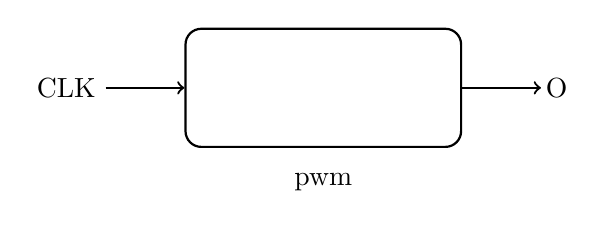
\begin{tikzpicture}
\draw node [draw,rectangle, minimum height=15mm, minimum width=35mm,rounded corners=2mm,thick](entity){};
\draw[->,thick] ($ (entity.west)-(10mm,0mm)$) -- ($ (entity.west) - (0mm,0mm)$);
\draw node at ($ (entity.west)-(15mm,0mm)$){CLK};

\draw[->,thick] (entity.east) -- ($ (entity.east) + (10mm,0)$);;
\draw node at ($ (entity.east) + (12mm,0)$){O};

\draw node at ($ (entity) - (0,12mm)$){pwm};

\end{tikzpicture}
\end{center}

Do not change the file "pwm.vhdl".
\\

The "pwm" entity shall generate a PWM (Pulse-Width Modulation) signal from a clock signal (input port CLK) with the following constraints:
\begin{itemize}
\item Period $T_{PWM}$ = %%PERIOD, frequency $f_{PWM}$= %%FRQ
\item Duty cycle $D_{PWM}$= %%DUTY
\item The signal lead edge has to be held fixed, the tail edge has to be modulated.
\end{itemize}
\vspace{0.3cm}

This behavior has to be programmed in the attached file "gates\_beh.vhdl".
\\

To be proper synthesizeable for a FPGA, the PWM signal generation has to be done without the VHDL constructs 'after' and 'wait'.
\\

To turn in your solution write an email to %%SUBMISSIONEMAIL with Subject "Result Task %%TASKNR" and attach your file "pwm\_beh.vhdl".

\vspace{0.7cm}

Good Luck and May the Force be with you.



\end{document}
